\section{Background and Motivation}
\label{sec:bkg}

Here, we provide a brief overview of our terminology, transformers, and xxx. We assume that the readers are generally familiar with how to train and inference
deep neural networks on NVIDIA GPUs.


% \subsection{Object Detection and xxx}

% The target of object detection is to predict a set of bounding boxes and labels for each substance in an image. Modern object detectors solve this problem 
% in a redundant way, by pre-defining a large set of proposals, anchors to address regression problem for the location of coordinates and classification problem 
% for the category labels. The performance of this model is significantly influenced by postprocessing steps to suffer from strong similarity predictions, by the
% design of deploymenting anchors and by the strategy that assign predicted boxes to anchors.

% \textbf{faster rcnn based approach}

% \textbf{detr based approach}

\begin{figure*}[htbp]
    \centering
    \label{fig:fig6}
    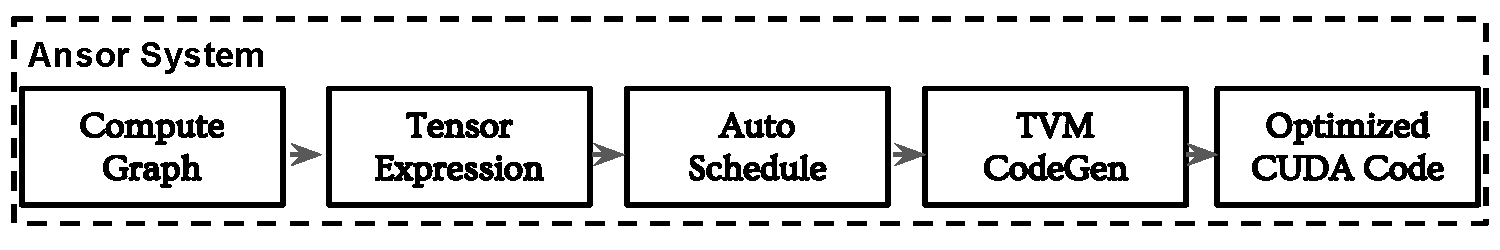
\includegraphics[height=3cm, width=15cm]{figs/fig6}
    \caption{The System Overview of Ansor. First, the input of Ansor is computation graph and it is converted into tensor expression language. Second, Auto-Schedule module
    can search the optimial schedule automatically for the tensor expression language. Finally, TVM code generation can generate optimized CUDA code on GPU backend 
    for the computation graph.}
\end{figure*}
\subsection{Image Recognition}
{\color{red} Image Classification, Object Detection, Semantic Segmentation}

Image recognition has been significantly boosted with the development of deep neural networks. There are three particularly important 
tasks in image recognition: (1) Image classification, (2) object detection, and (3) semantic segmentation. Image classification can classify what is contained in an image. Object detection is a combination of image location and classification. Image localization specifies the location of single object in an image whereas object detection specifies the location of multiple objects with their labels in the image. Image segmentation creates a pixel wise mask of each object in the image. Note that all popular approaches are still based on convolutional neural network where the feature encoding and extraction part are based on classical ConvNets like ResNet and VGG.

\subsection{Transfomers}

The transformer model, originally developed for a new attention-based building block for machine translation, or transforming an input sequence into an output 
sequence. Transformers build on a long sequence within natural language processing, most relevantly starting with word embeddings, neural machine translation, and 
sequence-to-sequence learning. The key element in transformer architecture is attention part, which is composed of neural networks layers that aggregate 
information from the entire input sequence and make model to learn to focus on particular parts of a sequence. One of the important advantages of attention-based model is their global computations and perfect memory scheduling, which leads them more eligible than 
RNNs on long sequences. Transformer models make two mian contributions. The first one is that it popularizes attention mechanisms to a particular module named 
\textit{multi-head attention}. The second one is that it does not rely on recurrent or convolutional algorithms, but completely relies on attention mechanisms. 
Most importantly, many similar architecture of subgraphs in transformer model can greatly reduce the tuning time for the kernel with the same configuration and run
parallelly, which we discuss below.

\textbf{Encoder:} The encoder module is composed of a stack of identical layers. There are two sub-layers in each layer. The first sub-layer is a multi-head 
attention mechanism, and the second sub-layer is a simple, positionwise fully dense layer. A residual connection layer is used between each of the two sub-layer
with a layer normalization. That is to say, the output of each sub-layer is actually the sum of the input and the attention of input under the layer normalization.
And the output of dimension is defined as $d_{model}$

\textbf{Decoder:} The structure of the encoder and decoder is very similar. The decoder is also composed of a stack identical layers. In addition to the two subl-layers
mentioned in the encoder module, a third sub-layer is inserted into the decoder module. The function of the third sub-layer is to perform multi-head attention over the 
output of the encoder part. At the same time, some modifications about masking mechanisms in the self-attention sub-layer is to prevent positions from attending to subsequent positions.
It combines with the fact that the output of embedding layers are offset by one position, and it is ensured that the perdiction of the \textit{i-}th position only 
depends on the known outputs less than the \textit{i-}th positions.

\textbf{Multi-head Attention:} Multi-head Attention generalizes attention mechanisms, and employs \textit{h} attention heads parallelly to get 
different learnt projections of a given sequence. Each attention head is an instance of \textit{scaled dot-product attention}, and takes queries (q),
keys (k), values (v) as its input. The function of attention is to find values corresponding to the keys closest to the input queries. The function of 
heads are also augmented with linear layers that project their inputs into a lower-dimensional space. The three inputs are first multiplied by weight
tensors \textit{wq}, \textit{wk}, \textit{wv}, respectively, as a learned input projection. The query and key tensors are subsequently multiplied together
and scaled, followed by applying the softmax operation in order to weight and select the most relevant results. This is then multiplied with \textit{vv} to 
produce the per-head output. The outputs of all the heads are finally concatenated and linearly projected back to the input dimensional size.
Multi-head attention may also have a masking step, which is used during the training stage to prevent the model from seeing the future information
and using message from a later part of a sequence. 



\textbf{Transformer Architecture:}
 A transformer architecture is composed of both encoder and decoder modules. It is worth noting that transformer-based model does not necessarily have 
decoder module. For instance, the widely used BERT model does not have this structure.


\subsection{Deep Learning Compiler}
\textbf{Ansor:} Ansor is equipped with a hierarhcical search space that decouples high-level structures and low-level details. 
Ansor constructs the search space for a computational graph automatically, 
eliminating the need to manually develop high-performance computing templates by the experienced engineers. 
It then uses auto-tuner to sample complete programs from the search space and implements fine-tuning on complete programs under the XGBoost cost model. 
Figure \ref{fig:fig6} shows the overall architecture of Ansor.




\subsection{Hierarchy of 2080Ti GPUs}
Compute Unified Device Architecture (CUDA) is a parallel computing platform and programmming model for GPUs, which exposes high-performance computing programmers
to the concepts of memory hierarchy and threads hierarchy. Accelerating deep learning performance on complex memory hierarchy needs to make good use of memory
units and compute units. 
\begin{figure}[htbp]
    \centering
    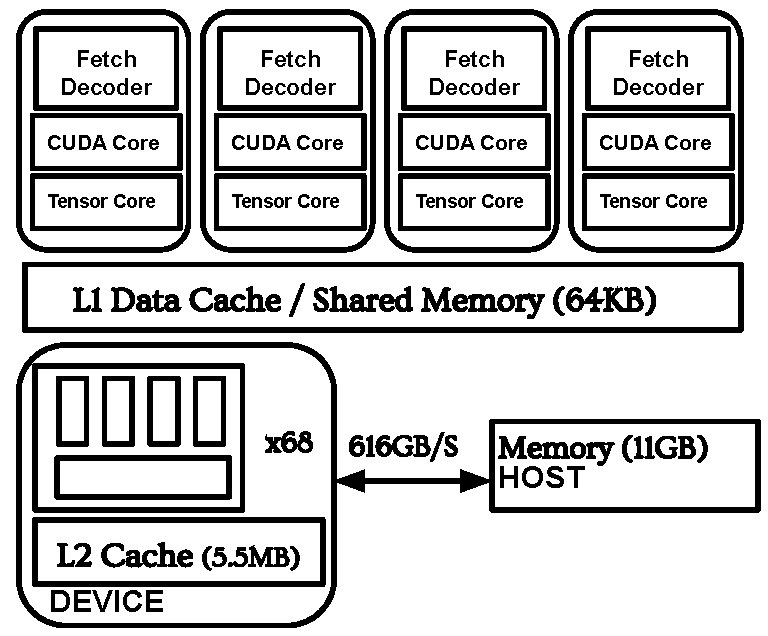
\includegraphics[height=5cm, width=6cm]{figs/fig5}
    \caption{A streaming multiprocessor and the architecture in GeForce RTX 2080 Ti GPU}
    \label{fig5}
\end{figure}
As shown in Figure \ref{fig5}, there are many programmable memories at different levels of GPU devices. GPU memory units are different from access pattern to management.
NVIDIA 2080Ti GPU contains 68 Stream Multiprocessors(SMs) which can run parallelly on the board. Each SM has its shared memory, which can be accessed by threads
in the same block. A SM is partitioned into multiple blocks and each block can only access its private shared memory. Registers and local memory can only be visited
by a single thread. If the size of the required memory is larger than the size each thread allocated, local memory in each block will be used. Generally, data copying
from host memory to device memory will be executed before the computation kernel is launched. \\
On-chip memory is fast and adjacent to chips whereas off-chip memory is slow and far away from chips. Different types of memory have different access patterns.
Registers and local memory in the same block are both private to each thread. Registers are on-chip with low latency. Shared memory is organized by a full-sized 
replica of banks. Simultaneous data accessing by different threads to the same bank will lead to a shared memory bank conflict problem, and it gives rise to
higher latency. 
% \textbf{\subsection{Challenges with End-to-End Optimization}}

